\chapter{SNMP}

\section{Inleiding}

SNMP staat voor het Simple Network Management Protocol. De naam vertelt je meteen al waarvoor het protocol dient: het beheren van je netwerk.
De 'S' van SNMP betekent niet simpel als in simpel in gebruik (alhoewel het niet moeilijk in gebruik is), maar dat het protocol zo simpel mogelijk gehouden is.
Met SNMP kun je allerhande informatie opvragen van allerhande soorten toestellen. In principe is er geen limiet op hetgeen je kunt opvragen,
maar de functionaliteit om die informatie op te vragen moet wel geïmplementeerd worden. Normaal gezien gebeurt dat door de fabrikant van het toestel.

Er zijn maar een paar voorwaarden om met behulp van SNMP informatie van een toestel op te kunnen vragen. Eerst en vooral moet het toestel natuurlijk SNMP ondersteunen.
Ze moet ook de functionaliteit bezitten om de gevraagde informatie te kunnen aanbieden en tenslotte moet de vrager ook kennis hebben van welke informatie
er allemaal opgevraagd kan worden. Zo zal een router niet dezelfde informatie kunnen aanbieden als bijvoorbeeld een switch. Er is wel een minimale
verzameling van gegevens die door alle toestellen ondersteund moet worden om als SNMP-compatibel bestempeld te kunnen worden. Denk hierbij aan de naam van het
systeem, hoe lang het systeem al online is, welke netwerkinterfaces ze heeft, enzovoort.

Er zijn een groot aantal use cases te bedenken voor het gebruik van SNMP maar hier zijn enkele van de belangrijkste.

\begin{itemize}
	\item Inventarisatie: met behulp van discovery procedures en SNMP kun je een overzicht krijgen van alle toestellen aangesloten op het netwerk,
	en vooral hoe ze met elkaar verbonden zijn. Netwerken zijn niet statisch: er worden toestellen toegevoegd en verwijderd. Met SNMP kun je een
	actueel beeld van de aangesloten hardware en netwerktopologie verkrijgen. Dit is zeer handig voor kleine en middelgrote netwerken, maar onmisbaar
	voor grote netwerken!
	
	\item Configuratiebeheer: voor wat betreft de hardwarekant overlapt dit eigenlijk met de inventarisatie. Maar voor de softwarekant kun je met SNMP de
	configuratieinstellingen van toestellen opvragen en controleren. Bijvoorbeeld: voor Windowstoestellen kun je de lijst opvragen van geïnstalleerde updates,
	van routers kun je de routetabel controleren en van switches de \gls{arptabel}.
	
	\item Performantiebeheer: ook de netwerkverzadiging kun je controleren met SNMP. Zo kun je de huidige toestand in de gaten houden,
	onregelmatigheden vaststellen en trends volgen. Op basis van deze trends kunnen dan plannen opgesteld worden voor toekomstige uitbreidingen
	van de netwerkcapaciteit op knelpunten.
\end{itemize}

Voor kleine netwerken kan SNMP het leven van een systeembeheerder een stuk gemakkelijker maken. Om grote netwerken te beheren is SNMP quasi een vereiste.
De conclusie is duidelijk: SNMP zou onderdeel moeten uitmaken van de gereedschapskit van elke systeembeheerder.


% SNMP meer in detail / bouwstenen/onderdelen van SNMP
% Aspecten van SNMP?

\section{SNMP meer in detail}
\todo{Betere titel?}

\subsection{De S van SNMP}
\todo{Betere titel?}

Zoals gezegd staat de 'S' van SNMP voor simple. Hiermee wordt vooral bedoeld dat men SNMP zo simpel mogelijk heeft gehouden.
De reden waarom dit zo is, is tweeledig: eenvoud van implementatie en met oog op performantie. % Voor het toestel, niet het netwerk!!!
Omdat SNMP zo simpel in elkaar steekt, kunnen fabrikanten zonder al te veel moeite SNMP implementeren op hun hardware.
Door de simpliciteit van SNMP moet er bovendien slechts weinig werk verricht worden om SNMP-requests te beantwoorden.
Zodoende kunnen zelfs toestellen met zeer zwakke hardware, zoals embedded systemen, ook SNMP ondersteunen.


% Componenten?
\subsection{Onderdelen van SNMP}
\todo{Betere titel?}

SNMP kent twee soorten toestellen: SNMP-agents en SNMP-managers. In het client-server principe wordt de serverrol verricht door de SNMP-agent
en de client door de SNMP-manager.

\begin{itemize}
	\item De SNMP-agent is een stuk software dat draait op de netwerkcomponenten en informatie bijhoudt over het toestel.
	Als iemand daar om vraagt zal de agent hem ook die informatie verstrekken.
	
	% De GLS Reset zorgt ervoor dat de afkorting zeker languit wordt uitgeschreven
	\item De SNMP-manager, vaak een \glsreset{nms} \gls{nms} genoemd, is de software die de SNMP-requests genereert, verstuurt naar de
	SNMP-agents en uiteindelijk de antwoorden verwerkt. Een \gls{nms} zal meestal niet één maar meerdere SNMP-agents van verschillende toestellen ondervragen.
	Aan de hand van de verkregen informatie kan de \gls{nms} beslissen om verdere acties uitvoeren.
\end{itemize}


\subsection{Uniformiteit}
\todo{Betere titel?}

Een van de grootste voordelen van SNMP is het feit dat ze je een uniforme manier aanbiedt om je netwerk te beheren. Fabrikanten van netwerkapparatuur
bieden graag hun eigen oplossing aan om hun toestellen te beheren, maar het probleem is dat netwerken slechts hoogst uitzonderlijk uit apparatuur
bestaan van slechts een fabrikant. De managementoplossingen van de ene fabrikant werken natuurlijk niet om ook de toestellen van de andere
fabrikant te beheren. Met SNMP zit je dus niet vast aan een fabrikant en kun je op uniforme wijze gans je netwerk beheren.

SNMP biedt maar weinig functionaliteit aan en dat speelt zowel in zijn voordeel als in zijn nadeel. \todo{Te lange zin?} Het voordeel is zoals eerder vermeld het
gemak waarmee fabrikanten SNMP kunnen implementeren, maar het nadeel is het gebrek aan features: met SNMP kun je enkel ruwe data opvragen.
Als je meer uit je data wenst te halen moet je die zelf achteraf verder verwerken. Denk aan het bijhouden van historische data, het combineren
van verschillende gegevens om verbanden te zien, grafieken opmaken of zelfs ganse rapporten opstellen. Die dingen worden wel ondersteund door de
managementoplossingen van fabrikanten, maar bij SNMP is het aan de gebruiker om die data uit de SNMP-gegevens te extraheren.


\subsection{Onderliggende protocols}

SNMP steunt op IP en UDP als transportprotocol. Dankzij de IP laag kan SNMP ook werken op heterogene netwerken.
UDP werd verkozen boven TCP vanwege de eenvoudige werking, wat weer handig is voor low-level netwerkcomponenten.
Bovendien heeft UDP een kleinere impact op het netwerkverkeer dan TCP\cite{moreau}.
Het nadeel van UDP is wel dat er geen bevestiging gebeurt van verstuurde pakketten.
Als er een pakket verloren gaat is het dan aan de \gls{nms} om dit te detecteren en op te vangen.
Normaal zal de \gls{nms} simpelweg de SNMP-query opnieuw versturen.
Voor het versturen en ontvangen van SNMP-berichten wordt er standaard gebruik gemaakt van poort 161.


\section{Object Identifiers}
\todo[inline]{Alinea's opsplitsen.}
Elk mogelijk soort gegeven dat je kunt opvragen van een toestel dat SNMP ondersteunt wordt wereldwijd uniek geïdentificeerd\cite{moreau} door een \gls{oid}.
\glspl{oid} worden hiërarchisch ingedeeld in een boomstructuur, net als bij DNS. De eindpunten van de boom stellen objecten voor en de knooppunten van de boom
worden gebruikt om objecten logisch te groeperen. De namen van de knooppunten bepalen de uiteindelijke \gls{oid}.
\glspl{oid} hebben een dotted-decimal notatie waarbij de knooppunten en het object van elkaar gescheiden worden door punten. %TODO Citatie?
Van links naar rechts wordt de \gls{oid} opgebouwd door het hoogste knooppunt tot het uiteindelijk object.
Een voorbeeld van een \gls{oid} die de uptime van een syteem teruggeeft is iso.org.dod.internet.mgmt.mib-2.system.sysUpTime.
Het stuk van de boomstructuur waarin die \gls{oid} valt kun je ook zien in figuur \ref{boomstructuur}.
De tekstuele notatie van een \gls{oid} valt zoals je ziet nogal lang uit en is moeilijk om te onthouden.
Daarom is het ook mogelijk om van een numerieke notatie gebruik te maken.
Elk knooppunt heeft behalve de tekstuele naam ook een volgnummer waar gebruik van kan gemaakt worden en een veel kortere \gls{oid} oplevert.
De \gls{oid} die hiervoor als voorbeeld werd gegeven wordt dan 1.3.6.1.2.1.1.3.
In de figuur van de boomvoorstelling staat het volgnummer van elk knooppunt ook tussen ronde haken. Eventueel kan er ook gebruik gemaakt worden van een
hybride notatie waarbij afwisselend gebruik kan gemaakt worden van de tekstuele of numerieke identificatie van een knooppunt.
Een mogelijke hybride voorstelling van het vorig voorbeeld is 1.3.6.1.mgmt.1.1.sysUpTime.

\begin{figure}[h]
	\centering
	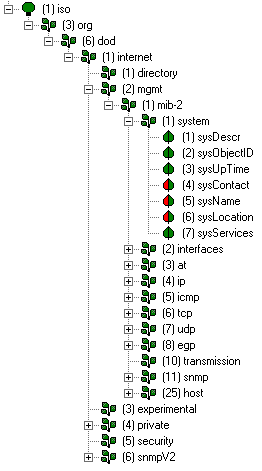
\includegraphics{figures/snmp/OID_tree}
	\caption{Boomstructuur van SNMP-objecten}
	\label{boomstructuur}
\end{figure}


\section{Management Information Base}
SNMP-agents houden een overzicht bij van alle gegevens die ze moeten bijhouden in een zogeheten \gls{mdb}.
In die \gls{mdb} zit een verzameling van \gls{mib} bestanden.\footnote{De \gls{mib}-bestanden worden eerst gecompileerd naar een binair formaat
alvorens ze in de \gls{mdb} opgeslagen worden.\cite{moreau}}
In die \gls{mib}-bestanden worden de eigenlijke SNMP-objecten gedefiniëerd. Vaak gaat men samenhorende objecten in een \gls{mib}-bestand samen stoppen.
Bijvoorbeeld alle objecten die bij een bepaald protocol horen, of alle objecten die worden geïmplementeerd door een bepaalde fabrikant.
Voor elk object wordt de naam en het volgnummer vastgelegd die zullen gebruikt worden in het OID voor dat object, alsook een beschrijving ervan en
van wat voor soort datastructuur er gebruik gemaakt wordt om de data voor te stellen (bv. een string of integer).

Ook voor \glspl{nms} zijn \gls{mib}-bestanden zeer belangrijk. Want ook zij moeten weten welke gegevens ze precies kunnen opvragen van een bepaalde
agent, en vooral: hoe ze die gegevens moeten interpreteren! Een \gls{nms} zal dus minstens over dezelfde \glspl{mib} moeten beschikken als de
agents die hij ondervraagt. Een groot aantal \glspl{mib} zijn gestandaardiseerd en worden ook standaard meegeleverd met SNMP-software.
Een aantal van die gestandaardiseerde \glspl{mib} moeten ook verplicht ondersteund worden door SNMP-agents om de stempel 'SNMP compatibel' te mogen dragen.
Het MIB-2 knooppunt die je kunt zien in figuur \ref{boomstructuur} is daar een voorbeeld van.
Die minimale set van gegevens zal je dus van ieder SNMP toestel kunnen opvragen.


\section{Tabellen}

Behalve scalaire waarden is het ook mogelijk om tabellen te gebruiken met SNMP.
We maken gebruik van de standaardtabel voor netwerkinterfaces \emph{ifTable} met als \gls{oid} 1.3.6.1.2.1.2.2 ter illustratie.
Een tabel wordt als volgt gedefiniëerd in een \gls{mib}-bestand: 
je hebt enerzijds een tabelobject (hier ifTable) en anderzijds een rijobject (hier ifEntry).
De definitie van het tabelobject zie je in \lstlistingnamesentence{} \ref{definitie-iftable}.
De volgende \lstlistingnamesentence{}en tonen de definities van de overige objecten.

Het tabelobject wordt gedefiniëerd als een sequentie of opeenvolging van rijobjecten.
Het rijobject wordt op zijn beurt gedefiniëerd als een sequentie van kolommen.
Hiervoor wordt een aparte sequentiedefinitie (IfEntry) gebruikt die 
bestaat uit een opeenvolging van kolomnamen gevolgd door hun datatype.

\begin{lstlisting}[language=asn.1, float=h, caption={Definitie van ifTable}, label=definitie-iftable]
ifTable OBJECT-TYPE
	SYNTAX	SEQUENCE OF IfEntry
	ACCESS	not-accessible
	STATUS	mandatory
	DESCRIPTION
			"A list of interface entries.  The number of
			entries is given by the value of ifNumber."
	::= { interfaces 2 }
\end{lstlisting}

\begin{lstlisting}[language=asn.1, float=h, caption={Sequentiedefinitie voor een tabelrij}, label=definitie-sequentie-rij]
IfEntry ::=
	SEQUENCE {
		ifIndex
			INTEGER,
		ifDescr
			DisplayString,
		ifType
			INTEGER,
		...
	}
\end{lstlisting}

Bij de definitie van het rijobject zelf zie je dat er als syntax (datatype) de voorgaande sequentiedefinitie wordt gebruikt.
Merk op dat de sequentiedefinitie (IfEntry) begint met een hoofdletter maar de definitie van het object zelf niet (ifEntry).

\begin{lstlisting}[language=asn.1, float=h, caption={Definitie van een rijobject}, label=definitie-rijobject]
ifEntry OBJECT-TYPE
	SYNTAX	IfEntry
	ACCESS	not-accessible
	STATUS	mandatory
	DESCRIPTION
			"An interface entry containing objects at the
			subnetwork layer and below for a particular
			interface."
	INDEX	{ ifIndex }
	::= { ifTable 1 }
\end{lstlisting}

Ook belangrijk is het INDEX-attribuut. Deze geeft aan hoe de tabel geïndexeerd moet worden, dus hoe je aan individuele rijen kunt geraken.
Dit kan een eenvoudige integer zijn of een samenstelling van kolommen die een rij uniek kan identificeren.
Hier wordt ifIndex gedefiniëerd als een eenvoudige integer.

\begin{lstlisting}[language=asn.1, float=h, caption={Definitie van ifIndex}, label=definitie-ifindex]
ifIndex OBJECT-TYPE
	SYNTAX	INTEGER
	ACCESS	read-only
	STATUS	mandatory
	DESCRIPTION
			"A unique value for each interface.  Its value
			ranges between 1 and the value of ifNumber.  The
			value for each interface must remain constant at
			least from one re-initialization of the entity's
			network management system to the next re-
			initialization."
	::= { ifEntry 1 }
\end{lstlisting}

De indexering gebeurt dan als volgt. Om te beginnen heb je de \gls{oid} van de tabel zelf: 1.3.6.1.2.1.2.2.
Het rijobject heeft ook een eigen \gls{oid}. Zijn volgnummer is 1 dus die komt achter de \gls{oid} van de tabel.
Daarna komt het volgnummer van de kolom. Laten we als voorbeeld de kolom met de snelheid van de interface nemen (ifSpeed).
Deze heeft als volgnummer 5. De \gls{oid} voor die kolom wordt dan 1.3.6.1.2.1.2.2.1.5.
Als we alle \glspl{oid} overlopen die beginnen met de \gls{oid} van de ifSpeed kolom, dan krijgen we de waarden van alle rijen voor die ene kolom.
Als we ook nog eens een specifieke rij willen opgeven dan volgt dat na de kolomaanduiding.
Vermits er hier gebruik gemaakt wordt van een simpele integer als index kunnen we achteraan de \gls{oid} 1 toevoegen om 
de snelheid van de \emph{eerste} interface te weten te komen. De uiteindelijke \gls{oid} wordt dan 1.3.6.1.2.1.2.2.1.5.1.
Je kunt dit visueel ook bevestigen in \figurenamesentence{} \ref{boomstructuur-tabel}.

Omdat de kolomaanduiding voor de rijaanduiding komt in een \gls{oid},
zal het overlopen van alle \glspl{oid} die beginnen met de \gls{oid} van de tabel tot resultaat hebben dat de tabel kolom per kolom wordt overlopen.
Deze operatie wordt een SNMP walk van een \gls{oid} genoemd en wordt later verder uitgelegd.

\begin{figure}[h]
	\centering
	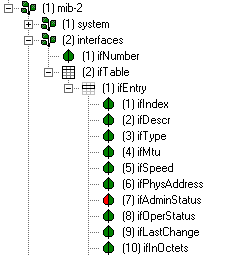
\includegraphics[resolution=110]{figures/snmp/ifTable-cropped}
	\caption{Boomstructuur van een tabel}
	\label{boomstructuur-tabel}
\end{figure}


\section{SNMP Operaties}
\label{snmp-operaties}
SNMP maakt gebruik van het \gls{pdu} berichtformaat voor al het communicatieverkeer tussen SNMP-agents en \glspl{nms}.
Er worden een aantal verschillende operaties ondersteund door SNMP en die hebben elk hun eigen \gls{pdu}-formaat\cite{essentialsnmp}.
Hieronder worden enkel de belangrijkste SNMP-operaties gegeven die relevant zijn voor de masterproef:

\begin{itemize}
	\item GET
	\item GETNEXT
	\item GETBULK
\end{itemize}


\subsection{GET}
De GET-operatie was de eerste en belangrijkste SNMP operatie.
De GET-operatie wordt geïnitieerd door de \gls{nms} en laat die toe om een gegeven van een SNMP-agent op te vragen.
Om te weten welk gegeven de \gls{nms} nu juist wenst te weten te komen geeft die een \gls{oid} mee met de \gls{pdu} die het gegeven uniek zal identificeren.
Herinner je dat zowel de SNMP-agent als \gls{nms} over dezelfde \gls{mib} beschikken die dat \gls{oid} definiëert zodat ze beiden perfect weten waarover het gaat.
De SNMP-agent ontvangt de \gls{pdu} en verwerkt deze. Een nieuw GET-response \gls{pdu} wordt opgesteld voor dat \gls{oid} met de waarde ervan ingevuld en
terug verstuurd door de SNMP-agent. De \gls{nms} ontvangt de GET-response \gls{pdu} en weet nu de waarde voor dat \gls{oid}.

\todo[inline]{Figuur?}


\subsection{GETNEXT}
De GETNEXT-operatie wordt gebruikt om een verzameling van opeenvolgende \glspl{oid} op te vragen.
Gegeven een bepaalde \gls{oid} zal de GETNEXT-operatie de eerstvolgende \gls{oid} met bijhorende waarde teruggeven.
Dit gebeurt in lexicografische volgorde en vermits \glspl{oid} samengesteld zijn door integers kan zo makkelijk een ganse boomtak overlopen worden.
Deze manier van werken noemt men diepte-eerst zoeken.\cite{essentialsnmp}
Wanneer de \gls{nms} het antwoord ontvangt van een GETNEXT-operatie zal ze een nieuwe sturen voor het volgende \gls{oid}.
De \gls{nms} zal blijven GETNEXT-\glspl{pdu} sturen tot dat de agent een foutmelding terugstuurt die aangeeft dat het einde van de \gls{mib} bereikt is.

Normaal gezien zal je niet rechtstreeks in contact komen GETNEXT-operaties, maar zul je gebruik maken van de SNMP walkopdracht.
Je hoeft enkel de OID mee te geven met de SNMP walkopdracht waarop deze de nodige GETNEXT-requests zal sturen om de ganse boomtak te overlopen.
\todo{Herhaalt eigenlijk wat er hierboven werd gezegd, maar ipv NMS -> SNMP Walk}

\todo[inline]{Figuur?}


\subsection{GETBULK}
Met de tweede versie van SNMP werd de GETBULK-operatie gespecificeerd.
Deze operatie laat je toe om in een request meteen een heleboel \glspl{oid} op te vragen.
Bij een gewone GET-operatie kun je ook meerdere \glspl{oid} meegeven maar de berichtgrootte wordt beperkt door de capaciteit van de SNMP-agent.
Als een SNMP-agent geen antwoord kan geven op alle \glspl{oid} die werden gevraagd in de GET-operatie wordt een foutboodschap teruggestuurd zonder data.
De GETBULK-operatie daarentegen probeert zo veel mogelijk data terug te sturen als het kan.
Met de GETBULK-operatie is het dus wel mogelijk om incomplete antwoorden terug te krijgen.\cite{essentialsnmp}

\section{Manieren om SNMP gegevens op te vragen}
\todo[inline]{Manieren/methoden/... om SNMP gegevens op te vragen. Of gewoon SNMP gegevens opvragen.}

Aan de hand van de SNMP operaties besproken in sectie \ref{snmp-operaties} zijn er
verschillende mogelijkheden om gegevens op te vragen.
\todo[inline]{Vul mij aan.}

\subsection{Enkelvoudige gegevens}
\todo{Goede titel? Enkelvoudig?}

Indien je maar geïnteresseerd bent in een gegeven dan ligt het voor de hand om gebruik te maken van de SNMP GET-operatie.
Voorwaarde is wel dat je exact de OID kent van het gegeven dat je wenst op te vragen.



\todo[inline]{Merk op dat je een .0 achteraan moet toevoegen om de waarde van een OID op te vragen (waarom?)! Zie pg 39 cursus \& boek. \\
Een GETNEXT kan interessant zijn om de eerste waarde van een tabel op te vragen als je de indexering niet kent.}


\subsection{Meervoudige gegevens}

\todo[inline]{In principe is het ook mogelijk om meerdere gegevens op te vragen met een GET/GETNEXT(?) request.
Maar ze is wel veel gevoeliger aan fouten: een fout en je krijgt géén gegevens terug.}

\subsubsection{SNMP walk}

\subsubsection{SNMP walk met behulp van GETBULK-requests}


\section{Versies}
Er zijn drie grote versies van SNMP die momenteel in gebruik zijn op netwerktoestellen: SNMPv1, SNMPv2c en SNMPv3.
Ondanks dat SNMPv3 de twee voorgaande versies opvolgt kun je nog steeds veel toestellen vinden die enkel met SNMPv2c of zelfs met SNMPv1 werken.
Opnieuw is er een afhankelijkheid van de fabrikant om voor de ondersteuning van SNMPv3 te zorgen.


\subsection{SNMPv1}
De eerste versie van SNMP dateert al van 1988 maar is soms toch nog te vinden als enige ondersteunde versie op een toestel.
Een van de grootste gebreken die deze versie kenmerkt is de beveiliging.
De originele versie van SNMP maakte gebruik van een zogeheten \emph{community string} om SNMP-requests te beveiligen.
Die string fungeerde in feite als een soort wachtwoord die in cleartext met ieder SNMP-request werd meegegeven\cite{snmp-wiki}.
Natuurlijk kan iedereen die de requests kan onderscheppen het wachtwoord gewoon uitlezen en zelf requests met dat wachtwoord versturen.
SNMP voorziet in de mogelijkheid om niet alleen data uit te lezen, maar ook om data aan te passen met behulp van de SNMP SET-operatie.
Vanwege de slechte beveiliging wordt de SET-operatie echter zo goed als nooit geïmplementeerd in de SNMP-agent zodat de operatie geen effect heeft.

\todo[inline]{Waarom werd deze versie geaccepteerd? Werd aanzien als tijdelijke oplossing.}


\subsection{SNMPv2c}
De tweede versie van SNMP introduceerde in 1993 \cite{snmp-versions} oorspronkelijk de GETBULK-operatie en een betere beveiliging.
De nieuwe beveiliging werd echter als te complex beschouwd en werd op veel plaatsen niet aanvaard.
SNMPv2c werd in 1996 \cite{snmp-versions} voorgesteld als een alternatief die de verbeteringen van SNMPv2 had maar de complexe beveiliging ervan achterwege liet
ten voordele van de community strings van SNMPv1.
Deze versie werd wel aanvaard door de gemeenschap en is nog steeds in gebruik op een groot aantal toestellen.
De GETBULK-operatie was een welkome toevoeging aan SNMP omdat ze een veel performanter alternatief bood voor de vele GETNEXT-operaties
die voorheen nodig waren om grote hoeveelheden gegevens op te vragen.

\todo[inline]{Cross-compatibility met vorige versie}


\subsection{SNMPv3}
De derde en laatste versie van SNMP werd geaccepteerd als een volwaardige internetstandaard in 2002 \cite{snmpv3} en
bracht de reeds lang gevraagde verbetering in beveiliging met zich mee.
Omdat de vorige versies van SNMP slecht beveiligd waren werd het protocol enkel gebruikt voor het monitoren van het netwerk en performantiebeheer.
Met de verbeterde beveilging in SNMPv3 kan SNMP eindelijk een veilig platform aanbieden om niet enkel je netwerk passief te beheren zoals voorheen,
maar ook actief te beheren door configuratiewijzigingen uit te voeren via SNMP.
SNMPv3 is echter op veel toestellen nog steeds niet aanwezig en zeker de SNMP SET-operatie wordt in de praktijk maar zelden geïmplementeerd.

\section{Berichtstructuur van SNMP}

\todo[inline]{Berichtstructuur van SNMP}